\documentclass[letterpaper,12pt,oneside]{book}
\usepackage[top=1in, left=0.9in, right=1.25in, bottom=1in]{geometry}
\usepackage[utf8]{inputenc}
\usepackage[T1]{fontenc}
\usepackage[spanish,es-nodecimaldot,es-tabla]{babel}
\usepackage{graphicx}
\usepackage{tikz} 
\usepackage{tocloft}
\graphicspath{{./figs/}}
\usepackage{setspace}
\usepackage{fancyhdr}



\begin{document}

    \begin{titlepage}
        \thispagestyle{empty}
        \begin{minipage}[c][0.17\textheight][c]{0.25\textwidth}
            \begin{center}
                
\includegraphics[width=3.5cm, height=3.5cm]{Escudo-UNAM.pdf}
            \end{center}
        \end{minipage}
        \begin{minipage}[c][0.195\textheight][t]{0.75\textwidth}
            \begin{center}
                \vspace{0.3cm}
                \textbf{\textsc{\large Universidad Nacional Aut\'onoma de M\'exico}}\\[0.5cm]
                \vspace{0.3cm}
                \hrule height2.5pt
                \vspace{.2cm}
                \hrule height1pt
                \vspace{1.2cm}
                \textbf{\textsc{\large Facultad de Ciencias}}\\[0.5cm] %
            \end{center}
        \end{minipage}

        \begin{minipage}[c][0.81\textheight][t]{0.25\textwidth}
            \vspace*{5mm}
            \begin{center}
                \hskip2.0mm
                \vrule width1pt height13cm 
                \vspace{5mm}
                \hskip2pt
                \vrule width2.5pt height13cm
                \hskip2mm
                \vrule width1pt height13cm \\
                \vspace{5mm}
                
\includegraphics[height=4.0cm]{Escudo-FCIENCIAS.pdf}
            \end{center}
        \end{minipage}
        \begin{minipage}[c][0.81\textheight][t]{0.75\textwidth}
            \begin{center}
                \vspace{0.5cm}

                {\large\scshape Caracterización de Parámetros Geométricos en Imagenes de Cadera en Personas Sometidas a Cirugía de Cadera en la UMAE Lomas Verdes IMSS}

                \vspace{2cm}            

                \textsc{\large Reporte de práctica profesional}\\[0.5cm]
                \textsc{\large para obtener el t\'itulo de:}\\[1.5cm]
                \textbf{\textsc{\Large Licenciado en Física Biomédica}}\\[2 cm]
                \textsc{\Large p r e s e n t a :}\\[0.5cm]
                \textbf{\textsc{\large {Diego Medel Garduño}}}\\[2cm]          

                \vspace{0.5cm}

                {\large\scshape Tutores:\\[0.3cm] {M en C. Griselda Adriana Cruz Priego}}\\[.2in]

                \vspace{0.5cm}

                \large{Ciudad Universitaria, CDMX,}{ }{2024}
            \end{center}
        \end{minipage}
    \end{titlepage}

    \frontmatter
    \chapter{Agradecimientos}

    \newpage

    \tableofcontents
    \mainmatter

    \chapter{Introducción}
    \section{Planteamiento del problema}
    \section{Justificación}
    

    

    \chapter{Marco Teórico}
    
    \section{Sistema óseo}

    \subsection{Generalidades}


    La estructura principal del sistema óseo son los huesos, definidos como tejido conectivo altamente especializado, que se distingue por la presencia de una matriz extracelular capaz de mineralizarse, este proceso se debe a la presencia del mineral fosfato de calcio en forma de \textbf{cristales de hidroxiapatita}, lo que da como resultado la formación de un tejido duro, capaz de proveer sosten y protección al cuerpo humano, y no solo eso, la presencia de estos minerales propician que los huesos seas depositos de calcio y fosfato, ayudando con la concentración en sangre de estos minerales, dando paso a una regulación que permite la homeostasis. 

    \vspace{10pt}


    Considerando al ser humano como objetivo de estudio, su sistema óseo le confiere no solo soporte, sino tambien protección a las cavidades en donde existe la presencia de organos vitales, de igual manera conforma la base mecanica que le permite desplazarse y moverse. Por otro lado, el sistemá óseo funge de manera hematopoyetica, es decir, produciendo células sanguineas.  

    \vspace{10pt}

    El tejido óseo esta constituido por dos organizaciones estructurales que poseen caracteristicas distintivas. En la superficie externa del hueso se encuentra una capa densa, compacta, que se denomina \textbf{hueso compacto}, por otro lado en el interior del hueso se observa una estructura discontinua, que presenta cavidades en forma de red, conformada por espiculas de tejido óseo definidas como trabeculas, la forma peculiar de esta estructura permite el paso de la medula ósea y de vasos sanguíneos que nutren al tejido óseo, cabe mencionar que parte del hueso compacto es la cavidad medular, que es una estructura tubular, en el centro del hueso, que no contiene trabeculas.


    \vspace{10pt}


    La medula ósea que se transporta por la cavidad medular de los huesos y por los espacios del hueso esponjoso esta compuesta por \textbf{médula ósea roja}, que se compone de células hematopoyeticas, que permiten la formación de globulos rojos, blancos y plaquetas, a su vez la medula ósea roja esta formada por una red de fibras y células reticulares que tienen la función de dar soporte a vasos y celulas en desarrollo. Lo anterior es valido en etapas tempranas del desarollo, al haber crecimiento, la demanda de producción de células sanguineas disminuye, y solo ciertos huesos quedan encargados del proceso de hematopoyesis, como el esternon y las crestas iliacas, en todos los demás huesos, la medula roja ósea se transforma en tejido adiposo y se demonina \textbf{medula ósea amarilla}.

    \vspace{10pt}


    \begin{figure}[h!]
        \centering
        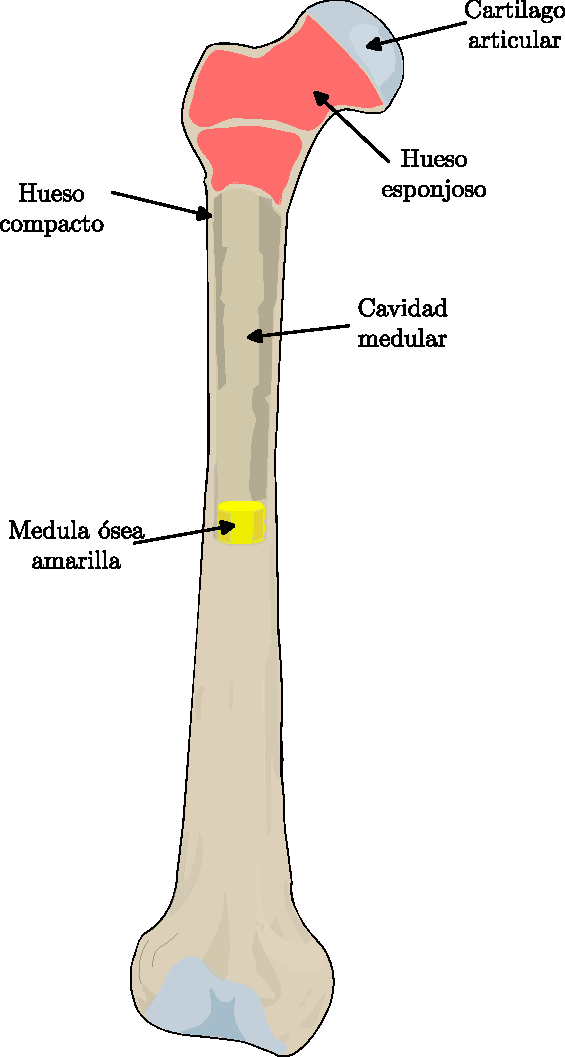
\includegraphics[scale = 0.60]{path1.pdf}
        \caption{Ejemplo de la anatomía de un hueso largo}
        \label{im1}
    \end{figure}

    \vspace{10pt}

    De manera anatomica el sistema óseo se divide en dos grandes grupos, el primero es el \textbf{esqueleto axial}, que comprende los huesos del craneo (neurocraneo y viscerocraneo), cuello y el tronco. Por otro lado el segundo grupo se denomina \textbf{esqueleto apendicular} y esta formado por los huesos de los miembros superiores e inferiores, tambien incluye los huesos de la cintura escapular y pélvica. A su vez los huesos dentro de esta división se discriminan por su forma y tamaño, de tal manera que existen un total de 4 tipos de huesos distintos: los huesos largos, que se caracterizan por presentar una forma tubular, los huesos cortos que son cuboideos y se encuentran solo en el tarso y el carpo, los huesos planos que se designan asi principalmente por su función de protección, sin embargo, dentro de su morfología sobresalen por tener muy poco espesor, por lo que tienen mayor cantidad de hueso compacto que de hueso esponjoso. La tercer clasificación son los huesos irregulares, los cuales no siguen un patron especifico en forma o función, pero si comparten no formar parte de ninguno de los otros grupos, por ultimo estan los huesos sesamoideos o tambien denominados huesos accesorio, estos se forman en consecuencia del uso excesivo de los tendones, por ejemplo la rotula de la rodilla conocida como patela. 


    \subsection{Histología del sistema óseo}

    \subsubsection{Estructura}



    Recapitulando, un hueso esta compuesto por dos clases de tejido, hueso esponjoso y hueso compacto, este ultimo en particular se encuentra conformado de manera estructural por complejos celulares en forma de laminillas concentricas a conductos especificos que permiten el paso de nervios y vasos sanguineos, conocidos como conductos de Havers o conductos osteónicos, esta unidad anatomofuncional del hueso compacto se conoce como osteona o sistemas de Havers. Es importante mencionar que las laminillas que se forman estan constituidas por matriz extracelular mineralizada, que en su interior posee distintas lagunas en donde se posan los osteocitos, que por su parte se alimentan del conducto ostenico a traves de conductillos. Los conductos osteonicos se encuentran comunicados con otros conductos osteonicos a traves de los conductos de Volkmann, la particularidad de estos conductos es que no se encuentran rodeados de laminillas concentricas de matriz extracelular, caractetistica importante para su distinción histologica. 

    \vspace{10pt}

    \begin{figure}[h!]
        \centering
        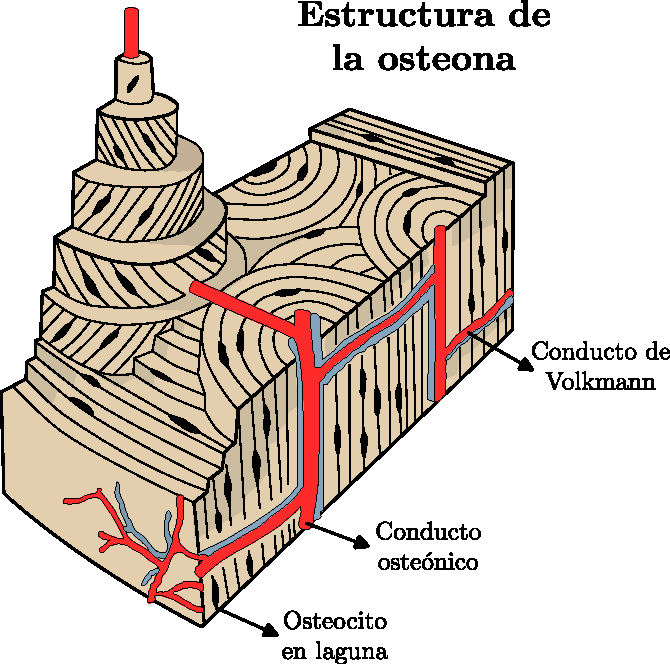
\includegraphics[scale = 0.65]{osteona.pdf}
        \caption{Estructura de una osteona}
        \label{im2}
    \end{figure}

    \vspace{10pt}

    Por su parte el hueso esponjoso comparte una estructura semejante con el hueso compacto, sin embargo, se diferencian por la distribución espacial ya que el hueso esponjoso se distribuye formando espiculas o trabeculas. La organización del tejido esponjoso le permite contener gran variedad de espacios medulares interconectados por donde pasa la medula ósea amarilla y roja. 

    \vspace{10pt}


    De manera superficial los huesos se encuentran rodeados por \textbf{periostio}, que se encuentra conformado por una capa externa de tejido conectivo denso fibroso y una capa interna de celulas osteoprogenitoras, el periostico cubre a los huesos casi en su totatilidad, ya que en las zonas donde el hueso se articula con otro ahi no hay tejido conectivo que recubra, sino se encuentra tejido cartilaginoso. Por otra parte las trabeculas del hueso esponjoso se encuentran cubiertas por una capa delgada de tejido fibroso especializado de manera externa, por su parte la capa interna es esta compuesta por celulas osteoprogenitoras (que pueden diferenciarse a osteoblastos) y celulas de revestimiento tambien denominadas como células endósticas.


    \subsubsection{Componente celular}

    Hasta el momento se ha hecho mención de los distintos tipo celulares que conforman al tejido oseo, sin embargo no se ha explicado a detalle cual es la función que desempeñan en en el hueso. De primera mano el tejido óseo se encuentra conformado por cinco tipos celulares: células osteoprogenitoras, osteobalastos, osteocitos, celulas de revestimiento óseo y osteoclastos.

    \vspace{10pt}

    \begin{itemize}
        \item \textbf{Células osteoprogenitoras}: Tambien denominadas células precursoras de osteoblastos, participan en primer lugar en la osteogénesis, la cual es el proceso de formación de nuevo tejido oseo. Este tipo celular se mantiene en reposo hasta que exista una via molecular que active su proceso de diferenciación con el que se transforma en osteoblastos y comienza a secretar matriz extracelular, por esta razón su principal lugar de alojamiento son en la superficie del tejido oseo ya sea en el periostio o en el endostio, tambien llegan a alojarse en los conductos de Havers y los conductos de Volkmann. 
        \item \textbf{Osteoblasto}: Por su función es denominada como célula osteoformadora, la cual tiene como función principal la secreción de colagena tipo 1 y proteinas de la matriz ósea, que constituyen al complejo inicial no mineralizado de la matriz extracelular, conocida como osteoide, entre las proteinas secretadas se encuentra la osteocalcina y la osteonectina, cuya papel esta implicado en la fijación de calcio, por otro lado se encuentran ciertas glucoproteínas de multiadhesión. \\ Otra de las funciones del osteoblasto es iniciar el proceso de calcificación, a partir de la secrecion de vesiculas matriciales.
        \item \textbf{Osteocito}: Despues de que el osteoblasto ha secretado la matriz osea suficiente para que este quede totalmente rodeado de ella, sus funciones del osteoblasto cambian y pasa a llamarse osteocito. Esta celula es responsable ahora de mantener la matriz ósea, para esto el osteocito participa en dos procesos la sintesis de matriz nueva y la degradación de la misma. \\ \\ La degradación esta relacionada con la muerte del osteocito, ya sea por traumatismos, vejez o apoptosis, lo que trae como concecuencia la resorción de la matriz ósea debia a la acción de los osteoclastos. Una vez que los osteoclastos finalizan el proceso de resorción de matriz celular, los osteoblastos se encargan del remodalo del tejido oseo. 
        \item \textbf{Células de revestimiento óseo}: Son células encargadas de tapizar tejido óseo que no esta siendo remodelado y son derivadas de los osteoblastos. Si la célula se encuentra revistiendo tejido superficial del hueso se les denomina como células periósticas, en cambio si se encuentran revistiendo la superficie interna se denominan células endósticas. \\ \\ El revestimiento superficial no es su unica función, tambien intervienen en el mantenimiento y nutrición de los osteocitos, por otro lado se encargan de regular el momiviento de minerales como el calcio y el fosfato de la sangre al hueso y viceversa. 
        \item \textbf{Osteoclastos}: Como ya se menciono, la función principal de los osteoclastos es la resorción ósea, proceso clave en para el mantenimiento homeostatico del calcio en el cuerpo. 
    \end{itemize}

 



    
    \section{Desequilibrio entre la sintesis y la resorción del tejido óseo}

    En la sección anterior se hizo mención de las funciones que desempeñan los osteoblastos y los osteoclastos, estos tipos célulares llevan a cabo la \textbf{remodelación ósea}, en la cual los osteoblastos se encargan de la formación de tejido óseo nuevo y los osteoclastos reabsorben el tejido preexistente, de esta manera se cumplen dos objetivos especificos, el primero de ellos consiste en la reparación de microlesiones en los huesos, para poder conservar la fuerza del sistema esqueletico, el segundo objetivo cumple con proveer al cuerpo la  concentración serica del ion calcio. 

    \vspace{10pt}

    El hueso humano alcanza su maxima cantidad de masa ósea cuando es adulto, la literatura refiere que gran parte de esta masa ósea se obtiene en la pubertad por acción de las hormonas sexuales secretadas en este periodo, aunque es importante esclarecer que la magnitud de la masa ósea maxima esta determinada por aspectos geneticos. Cuando se alcanza la masa ósea maxima, el cuerpo mantiene un equilibrio entre el tejido oseo que se reabsorbe y el que se crea, sin embargo, al pasar de los años y por diversos factores este equilibrio puede verse afectado. El caso a discutir en esta sección es cuando el desequilibrio se inclina hacia la resorción ósea, es decir, se esta reabsorbiendo más tejido óseo del que se esta creando, lo cual tiene distintas etiologias, ya que puede ocurrir que exista una disminución en la actividad osteoblastica, o que haya un aumento en la actividad osteoclastica o por otro lado exista un aumento en los sitios de remodelación ósea. Si el desequilibrio entre la resorción y producción de tejido óseo llega a afectar la arquitectura ósea, los huesos presentan daño a tal escala que se considera como irreparable, por lo que aumenta la fragilidad ósea y el riesgo de fractura, a esta afección se le conoce como \textbf{osteoporosis}

    \vspace{10pt}

    La osteoporosis se puede presentar por distintos factores, los principales estan definidos por hormonas regulatorias, que al sufrir algun tipo de desbalance este se ve reflejado en la calidad de hueso, ya que puede haber perdida de la masa ósea maxima, esta perdida puede ser reparable cuando el daño no es capaz de afectar la aquitectura del hueso, cuando la resorción destruye la corteza y llega al tejido esponjoso del hueso la velocidad en la que hay perdida ósea aumenta, de igual forma se afecta la conectividad trabecular del hueso, lo que en primer instancia provoca la formación de mayor cantidad de tejido poroso y por otro lado existe una disminución de la fortaleza biomecanica, lo que aumenta la pobabilidad de sufrir alguna caida. 

    \vspace{10pt} 

    Algunas de las hormonas que tienen una regulación en la remodelación osea, moderando la velocidad en la que se activan nuevos sitios de remodelación son los estrogenos, androgenos, la vitamina D, la hormona paratiroidea (PTH), ciertos factores de crecimiento como el IGF-I, IGH-II, TGF-$\beta$ y miembros de la superfamilia del factor de necrosis (TNF). La remodelación ósea consiste en una resorción ósea encargada por los osteoclastos seguida de un periodo de reparación, en el cual los osteoblastos se encargan de sintetizar tejido óseo nuevo.  

    \vspace{10pt}






    
    


    \section{Fracturas del femúr proximal}

    \chapter{Objetivos}
    \chapter{Materiales y Métodos}

    \chapter{Resultados}
    \chapter{Discusión de Resultados}
    \chapter{Conclusiones}

\end{document}